\documentclass[11pt,a4paper]{article}

%% ── Packages ────────────────────────────────────────────────────
\usepackage[utf8]{inputenc}
\usepackage[T1]{fontenc}
\usepackage{lmodern}
\usepackage[margin=2cm]{geometry}
\usepackage{amsmath,amssymb}
\usepackage{booktabs}
\usepackage{array}
\usepackage{enumitem}
\usepackage{float}
\usepackage[section]{placeins}
\usepackage{microtype}
\usepackage{titlesec}
\titlespacing*{\section}{0pt}{1.8ex plus 0.5ex minus 0.3ex}{1.0ex plus 0.2ex}
\titlespacing*{\subsection}{0pt}{1.4ex plus 0.4ex minus 0.2ex}{0.6ex plus 0.1ex}
\usepackage{pgfplots}
\pgfplotsset{compat=1.18}
\usepackage{tikz}
\usetikzlibrary{calc}
\usepackage{colortbl}
\usepackage[most]{tcolorbox}
\usepackage{xcolor}
\usepackage[colorlinks=true,linkcolor=blue!70!black,
  citecolor=green!50!black,urlcolor=blue!60!black]{hyperref}

%% ── Colours ─────────────────────────────────────────────────────
\definecolor{cblue}{HTML}{4472C4}
\definecolor{corange}{HTML}{ED7D31}
\definecolor{cgray}{HTML}{A5A5A5}
\definecolor{cgreen}{HTML}{228B22}
\definecolor{cred}{HTML}{CC0000}
\definecolor{cyellow}{HTML}{CC8800}
\definecolor{cpurple}{HTML}{7030A0}

%% ── Heatmap cell shortcuts ──────────────────────────────────────
\newcommand{\cfull}{\cellcolor{cgreen!35}\checkmark}
\newcommand{\cpart}{\cellcolor{cyellow!30}$\sim$}
\newcommand{\cnone}{\cellcolor{cred!15}$\times$}

%% ── tcolorbox styles ───────────────────────────────────────────
\newtcolorbox{finding}[1][]{%
  enhanced,
  colback=blue!4!white,
  colframe=cblue,
  coltitle=white,
  fonttitle=\bfseries\sffamily,
  title={Key Finding},
  attach boxed title to top left={yshift=-2mm, xshift=4mm},
  boxed title style={colback=cblue, sharp corners},
  sharp corners=south, rounded corners=north,
  boxrule=0.7pt,
  left=5pt, right=5pt, top=4pt, bottom=4pt,
  #1
}

\newtcolorbox{pattern}[1][]{%
  enhanced,
  colback=green!4!white,
  colframe=cgreen,
  coltitle=white,
  fonttitle=\bfseries\sffamily,
  title={Behavioural Pattern},
  attach boxed title to top left={yshift=-2mm, xshift=4mm},
  boxed title style={colback=cgreen, sharp corners},
  sharp corners=south, rounded corners=north,
  boxrule=0.6pt,
  left=5pt, right=5pt, top=4pt, bottom=4pt,
  #1
}

\newtcolorbox{failure}[1][]{%
  enhanced,
  colback=red!4!white,
  colframe=cred,
  coltitle=white,
  fonttitle=\bfseries\sffamily,
  title={Critical Failure Mode},
  attach boxed title to top left={yshift=-2mm, xshift=4mm},
  boxed title style={colback=cred, sharp corners},
  sharp corners=south, rounded corners=north,
  boxrule=0.6pt,
  left=5pt, right=5pt, top=4pt, bottom=4pt,
  #1
}

%% ═══════════════════════════════════════════════════════════════
\title{%
  \textbf{Performance Analysis of Repeated LLM Attempts\\
  at a Research-Level Mathematics Problem}
}
\author{Bartosz Naskr\k{e}cki\\
  {\normalfont\small (co-generated with Claude Code)}}
\date{}

%% ── Tighten float spacing ──────────────────────────────────────
\setlength{\floatsep}{6pt plus 2pt minus 2pt}
\setlength{\textfloatsep}{8pt plus 2pt minus 2pt}
\setlength{\intextsep}{6pt plus 2pt minus 2pt}
\setlength{\abovecaptionskip}{5pt}
\setlength{\belowcaptionskip}{2pt}

\begin{document}
\maketitle

%% ────────────────────────────────────────────────────────────────
\begin{abstract}
We analyse eleven independent attempts by a large language model
(LLM) to solve a research-level problem in arithmetic algebraic
geometry. The problem requires computing an exact large integer
through a chain of seven conceptual steps (S1--S7), each demanding
distinct mathematical insight. All eleven attempts were run
independently under identical conditions. Only \textbf{1 of 11}
attempts produced
the correct answer. Yet the collective knowledge across all
attempts covers the majority of the solution space---a striking
illustration of the \emph{last-mile problem} in AI mathematical
reasoning. This report presents anonymised performance metrics,
token-budget allocation patterns, solution-step discovery rates,
and behavioural observations, without disclosing the specific
mathematical techniques involved.
\end{abstract}

\smallskip
\noindent{\small\textbf{Acknowledgements.}
This analysis was generated and operationalised by Bartosz
Naskr\k{e}cki, based on reports from Epoch~AI regarding the
solutions of a FrontierMath Tier~4 problem submitted by the author.
The report is fully anonymised to remove all critical details of the
solution and was approved by Epoch~AI for public view.}

\tableofcontents

%% ═══════════════════════════════════════════════════════════════
\section{Experimental Setup}\label{sec:setup}

\subsection{Problem characterisation}

The target problem is drawn from a research-level mathematical
competition. It asks for the exact value of a summation over a
family of algebraic objects. The answer is a large integer. The official
solution proceeds through \textbf{seven key steps}, labelled
\textbf{S1}--\textbf{S7}, described only by their conceptual role:

\begin{enumerate}[label=\textbf{S\arabic*.},leftmargin=2.5em]
  \item \textbf{Structural decomposition}: Identify a relevant
    lower-dimensional structure.
  \item \textbf{Invariant computation}: Determine a key numerical
    invariant of the objects.
  \item \textbf{Deep geometric structure}: Recognise that the objects
    belong to a special class.
  \item \textbf{Associated objects}: Derive explicit auxiliary objects.
  \item \textbf{Counting formula}: Express the count in terms of data
    of the auxiliary objects.
  \item \textbf{Constraint classification}: Determine which subsets
    satisfy the problem's constraints.
  \item \textbf{Global cancellation}: Use symmetry to simplify the
    final calculation.
\end{enumerate}

\subsection{Experimental conditions}

\begin{itemize}[nosep]
  \item \textbf{Model}: A frontier LLM with code-execution
    capabilities.
  \item \textbf{Iterations}: 11 independent runs under identical
    conditions, labelled Iter\,1--10 and Final.
  \item \textbf{Token budget}: Each run used ${\sim}100$K+ reasoning
    tokens.
  \item \textbf{Isolation}: No inter-iteration memory; each of the 11
    runs started from scratch.
  \item \textbf{Transcript lengths}: 1\,909--3\,235 lines per
    iteration; 26\,128 lines total across Iter\,1--10.
\end{itemize}


%% ═══════════════════════════════════════════════════════════════
\section{Overall Performance}\label{sec:performance}

\subsection{Solution quality scores}

Each attempt is scored on a 0--7 scale: 1~point per solution step
fully discovered, 0.5~points for partial discovery.

\begin{figure}[H]
\centering
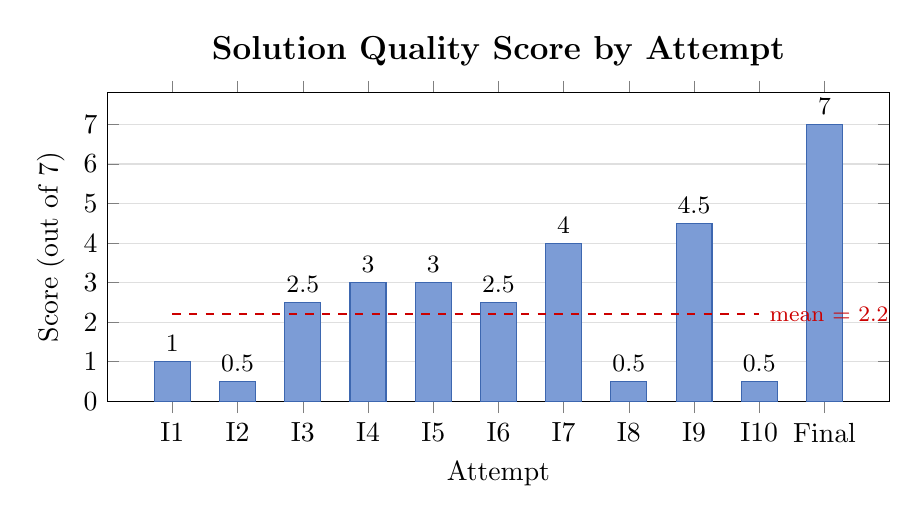
\begin{tikzpicture}
\begin{axis}[
    ybar,
    bar width=13pt,
    width=0.95\textwidth,
    height=5.5cm,
    ylabel={Score (out of 7)},
    xlabel={Attempt},
    symbolic x coords={I1,I2,I3,I4,I5,I6,I7,I8,I9,I10,Final},
    xtick=data,
    ymin=0, ymax=7.8,
    ytick={0,1,2,3,4,5,6,7},
    ymajorgrids=true,
    grid style={gray!25},
    nodes near coords,
    every node near coord/.append style={font=\small\bfseries},
    title={\textbf{Solution Quality Score by Attempt}},
    title style={font=\large},
]
\addplot[fill=cblue!70, draw=cblue!90!black] coordinates {
    (I1,1) (I2,0.5) (I3,2.5) (I4,3) (I5,3)
    (I6,2.5) (I7,4) (I8,0.5) (I9,4.5) (I10,0.5)
    (Final,7)
};
\draw[dashed, cred, thick]
    ({axis cs:I1,0}|-{axis cs:I1,2.2}) -- ({axis cs:I10,0}|-{axis cs:I10,2.2})
    node[right, font=\footnotesize, text=cred] {mean = 2.2};
\end{axis}
\end{tikzpicture}
\caption{Solution quality scores. The dashed line marks the mean of
  Iter\,1--10 (2.2/7). Only the Final attempt achieves a perfect
  score.}
\label{fig:scores}
\end{figure}

\begin{table}[H]
\centering
\caption{Score distribution (Iter\,1--10).}
\label{tab:score-stats}
\begin{tabular}{@{}lr@{}}
\toprule
\textbf{Statistic} & \textbf{Value} \\
\midrule
Mean & 2.20 / 7 \\
Median & 2.50 / 7 \\
Standard deviation & 1.42 \\
Minimum & 0.5 (Iters 2, 8, 10) \\
Maximum & 4.5 (Iter 9) \\
\bottomrule
\end{tabular}
\end{table}


\subsection{Submission types and correctness}

Submissions fell into three categories: \emph{code} (executable
algorithm), \emph{heuristic} (numerically interpolated guess), and
\emph{zero} (conjectured trivial answer).

\begin{table}[H]
\centering
\caption{Submission types: count, mean score, and correctness.}
\label{tab:types}
\begin{tabular}{@{}lcccl@{}}
\toprule
\textbf{Type} & \textbf{Count} & \textbf{Mean score}
  & \textbf{Correct} & \textbf{Attempts} \\
\midrule
Code      & 6 & 3.4 / 7 & 1 & I4, I5, I6, I7, I9, Final \\
Heuristic & 3 & 0.7 / 7 & 0 & I1, I8, I10 \\
Zero      & 2 & 0.5 / 7 & 0 & I2, I3 \\
\bottomrule
\end{tabular}
\end{table}

\begin{finding}
Of 11 attempts, only the Final Solution produced the correct answer,
and it did so via executable code---not analytic derivation. The
three heuristic guesses all overestimated the answer by 6.4--6.8\%,
suggesting a shared systematic bias in the estimation heuristic.
The two zero-submissions arose from a specific conceptual error:
confusing the vanishing of one component of the answer with the
emptiness of the feasible parameter set.
\end{finding}


%% ═══════════════════════════════════════════════════════════════
\section{Solution Step Discovery}\label{sec:steps}

\subsection{Aggregate discovery rates}

Figure~\ref{fig:discovery} shows how many of the 11 attempts fully
or partially discovered each of the seven solution steps.

\begin{figure}[H]
\centering
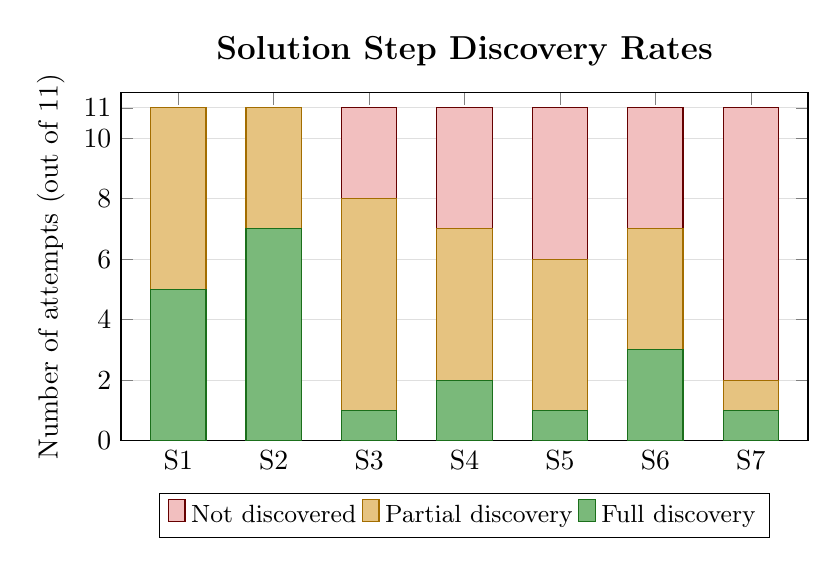
\begin{tikzpicture}
\begin{axis}[
    ybar stacked,
    bar width=20pt,
    width=0.85\textwidth,
    height=6cm,
    ylabel={Number of attempts (out of 11)},
    symbolic x coords={S1,S2,S3,S4,S5,S6,S7},
    xtick=data,
    ymin=0, ymax=11.5,
    ytick={0,2,4,6,8,10,11},
    ymajorgrids=true,
    grid style={gray!25},
    title={\textbf{Solution Step Discovery Rates}},
    title style={font=\large},
    legend style={at={(0.5,-0.15)}, anchor=north, legend columns=3,
      font=\small},
    reverse legend,
]
\addplot[fill=cgreen!60, draw=cgreen!80!black]
  coordinates {(S1,5)(S2,7)(S3,1)(S4,2)(S5,1)(S6,3)(S7,1)};
\addplot[fill=cyellow!50, draw=cyellow!80!black]
  coordinates {(S1,6)(S2,4)(S3,7)(S4,5)(S5,5)(S6,4)(S7,1)};
\addplot[fill=cred!25, draw=cred!50!black]
  coordinates {(S1,0)(S2,0)(S3,3)(S4,4)(S5,5)(S6,4)(S7,9)};
\legend{Full discovery, Partial discovery, Not discovered}
\end{axis}
\end{tikzpicture}
\caption{Stacked discovery rates for each solution step.
  Steps S1--S2 are universally attempted; S7 is discovered fully by
  only 1 of 11 attempts.}
\label{fig:discovery}
\end{figure}


\subsection{Per-attempt heatmap}

Table~\ref{tab:heatmap} provides a detailed per-step, per-attempt
breakdown.

\begin{table}[H]
\centering
\caption{Solution step discovery heatmap.
  \cfull\,= full,
  \cpart\,= partial,
  \cnone\,= not discovered.}
\label{tab:heatmap}
\small
\setlength{\tabcolsep}{4.5pt}
\begin{tabular}{@{}l*{11}{c}@{}}
\toprule
 & \rotatebox{70}{Iter\,1}
 & \rotatebox{70}{Iter\,2}
 & \rotatebox{70}{Iter\,3}
 & \rotatebox{70}{Iter\,4}
 & \rotatebox{70}{Iter\,5}
 & \rotatebox{70}{Iter\,6}
 & \rotatebox{70}{Iter\,7}
 & \rotatebox{70}{Iter\,8}
 & \rotatebox{70}{Iter\,9}
 & \rotatebox{70}{Iter\,10}
 & \rotatebox{70}{Final} \\
\midrule
\textbf{S1}
  & \cpart & \cpart & \cpart & \cfull & \cfull
  & \cpart & \cfull & \cpart & \cfull & \cpart & \cfull \\
\textbf{S2}
  & \cpart & \cpart & \cfull & \cfull & \cfull
  & \cfull & \cfull & \cpart & \cfull & \cpart & \cfull \\
\textbf{S3}
  & \cpart & \cnone & \cpart & \cpart & \cpart
  & \cpart & \cpart & \cnone & \cpart & \cnone & \cfull \\
\textbf{S4}
  & \cnone & \cnone & \cpart & \cpart & \cpart
  & \cpart & \cpart & \cnone & \cfull & \cnone & \cfull \\
\textbf{S5}
  & \cnone & \cnone & \cnone & \cpart & \cpart
  & \cpart & \cpart & \cnone & \cpart & \cnone & \cfull \\
\textbf{S6}
  & \cnone & \cnone & \cpart & \cpart & \cpart
  & \cpart & \cfull & \cnone & \cfull & \cnone & \cfull \\
\textbf{S7}
  & \cnone & \cnone & \cpart & \cnone & \cnone
  & \cnone & \cnone & \cnone & \cnone & \cnone & \cfull \\
\midrule
\textbf{Score}
  & 1 & 0.5 & 2.5 & 3 & 3
  & 2.5 & 4 & 0.5 & 4.5 & 0.5 & \textbf{7} \\
\bottomrule
\end{tabular}
\end{table}

\begin{pattern}[title={Phase-transition at S3}]
Steps S1 and S2 are at least partially discovered by all 11 attempts
(100\% engagement). Starting from S3, a sharp drop-off occurs:
3~attempts miss S3 entirely, and 9 of 11 miss S7. The transition
from ``surface-level analysis'' (S1--S2) to ``deep structural
insight'' (S3--S7) represents a qualitative barrier the model
rarely crosses fully.
\end{pattern}


%% ═══════════════════════════════════════════════════════════════
\section{Token Budget Allocation}\label{sec:tokens}

Each iteration's token expenditure was classified into five phases:
\emph{symbolic manipulation} (algebraic transformations),
\emph{empirical testing} (small-case experiments),
\emph{structural analysis} (geometric reasoning),
\emph{algorithm development} (code writing), and
\emph{planning \& hedging} (strategy deliberation, uncertainty
expression).

\begin{figure}[H]
\centering
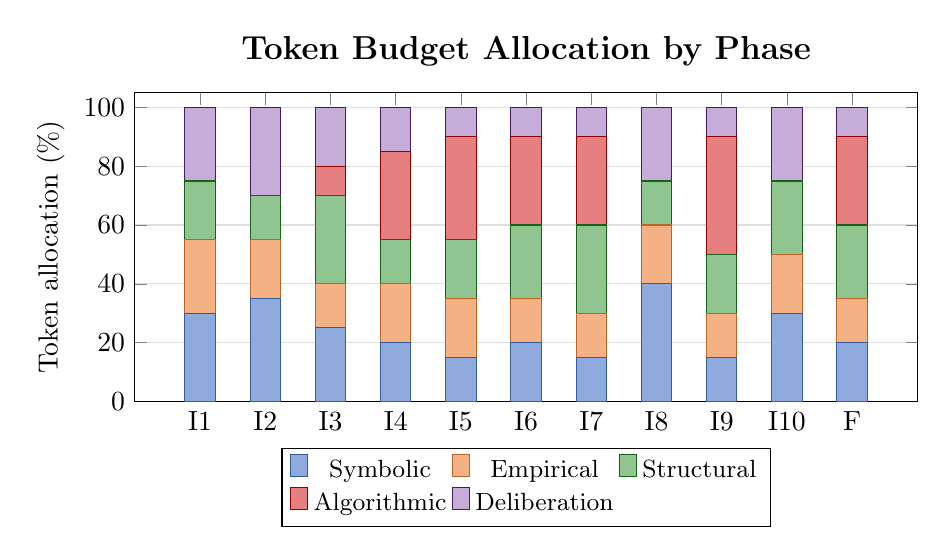
\begin{tikzpicture}
\begin{axis}[
    ybar stacked,
    bar width=11pt,
    width=0.95\textwidth,
    height=5.5cm,
    ylabel={Token allocation (\%)},
    symbolic x coords={I1,I2,I3,I4,I5,I6,I7,I8,I9,I10,F},
    xtick=data,
    ymin=0, ymax=105,
    ytick={0,20,40,60,80,100},
    ymajorgrids=true,
    grid style={gray!25},
    title={\textbf{Token Budget Allocation by Phase}},
    title style={font=\large},
    legend style={at={(0.5,-0.15)}, anchor=north, legend columns=3,
      font=\small},
]
\addplot[fill=cblue!60, draw=cblue!80!black] coordinates {
    (I1,30)(I2,35)(I3,25)(I4,20)(I5,15)(I6,20)(I7,15)(I8,40)(I9,15)(I10,30)(F,20)
};
\addplot[fill=corange!60, draw=corange!80!black] coordinates {
    (I1,25)(I2,20)(I3,15)(I4,20)(I5,20)(I6,15)(I7,15)(I8,20)(I9,15)(I10,20)(F,15)
};
\addplot[fill=cgreen!50, draw=cgreen!70!black] coordinates {
    (I1,20)(I2,15)(I3,30)(I4,15)(I5,20)(I6,25)(I7,30)(I8,15)(I9,20)(I10,25)(F,25)
};
\addplot[fill=cred!50, draw=cred!70!black] coordinates {
    (I1,0)(I2,0)(I3,10)(I4,30)(I5,35)(I6,30)(I7,30)(I8,0)(I9,40)(I10,0)(F,30)
};
\addplot[fill=cpurple!40, draw=cpurple!60!black] coordinates {
    (I1,25)(I2,30)(I3,20)(I4,15)(I5,10)(I6,10)(I7,10)(I8,25)(I9,10)(I10,25)(F,10)
};
\legend{Symbolic, Empirical, Structural, Algorithmic, Deliberation}
\end{axis}
\end{tikzpicture}
\caption{Approximate token budget allocation across all attempts.
  Code-submitting iterations (I4--I7, I9, Final) allocate 30--40\%
  to algorithm development, while non-code iterations spend 25--30\%
  on deliberation and hedging.}
\label{fig:tokens}
\end{figure}

\begin{finding}[title={Code investment correlates with score}]
Iterations that allocated ${\geq}30\%$ of tokens to algorithm
development (Iters~4, 5, 6, 7, 9, Final) achieved a mean score of
\textbf{3.4/7}. Those that allocated $0\%$ (Iters~1, 2, 8, 10)
achieved a mean of \textbf{0.6/7}---a factor of \textbf{5.7$\times$}
difference. The act of writing code, even incorrect code, appears
to force more rigorous structural reasoning.
\end{finding}


%% ═══════════════════════════════════════════════════════════════
\section{Strategic Diversity}\label{sec:strategies}

After a shared initial phase (algebraic decomposition and
small-case experiments, consuming ${\sim}20{-}30\%$ of tokens),
iterations diverged into five broad strategies:

\begin{enumerate}[label=\textbf{M\arabic*.},leftmargin=2.5em]
  \item \textbf{Analytic decomposition}: Express the count using
    tools from analytic number theory.
  \item \textbf{Structural identification}: Recognise that the object
    decomposes into a product of simpler components.
  \item \textbf{Parameter-space reasoning}: Use dimension arguments
    over the parameter space to constrain invariants.
  \item \textbf{Numerical extrapolation}: Interpolate from small-case
    data to guess the answer.
  \item \textbf{Classification-based filtering}: Classify auxiliary
    objects by discrete invariants to determine the feasible set.
\end{enumerate}

\begin{table}[H]
\centering
\caption{Strategy adoption by attempt (\textbullet\ = used).}
\label{tab:strategies}
\small
\setlength{\tabcolsep}{4pt}
\begin{tabular}{@{}l*{11}{c}@{}}
\toprule
 & \rotatebox{70}{Iter\,1}
 & \rotatebox{70}{Iter\,2}
 & \rotatebox{70}{Iter\,3}
 & \rotatebox{70}{Iter\,4}
 & \rotatebox{70}{Iter\,5}
 & \rotatebox{70}{Iter\,6}
 & \rotatebox{70}{Iter\,7}
 & \rotatebox{70}{Iter\,8}
 & \rotatebox{70}{Iter\,9}
 & \rotatebox{70}{Iter\,10}
 & \rotatebox{70}{Final} \\
\midrule
M1: Analytic
  & $\bullet$ & & & $\bullet$ & $\bullet$ & & & & $\bullet$
  & & $\bullet$ \\
M2: Structural
  & & & $\bullet$ & $\bullet$ & $\bullet$ & $\bullet$ & $\bullet$
  & & $\bullet$ & & $\bullet$ \\
M3: Parameter
  & & $\bullet$ & $\bullet$ & & & $\bullet$ & & $\bullet$
  & & $\bullet$ & \\
M4: Numerical
  & $\bullet$ & & & & & & & $\bullet$ & & $\bullet$ & \\
M5: Classification
  & & & & $\bullet$ & $\bullet$ & & $\bullet$ & & $\bullet$
  & & $\bullet$ \\
\midrule
\textbf{Count}
  & 2 & 1 & 2 & 3 & 3 & 2 & 2 & 2 & 3 & 2 & 3 \\
\bottomrule
\end{tabular}
\end{table}

The three highest-scoring independent iterations (Iter\,7:
score~4, Iter\,9: score~4.5, Iter\,4: score~3) all employed at
least three strategies simultaneously, including both M2
(structural identification) and M5 (classification-based
filtering)---the combination closest to the official solution.


%% ═══════════════════════════════════════════════════════════════
\section{Behavioural Patterns}\label{sec:behaviour}

\subsection{The last-mile problem}

\begin{failure}
The most striking pattern is the \emph{last-mile failure}: every
independent iteration discovers substantial fragments of the
solution but cannot assemble them into a complete, correct
computation. Across all 11 attempts:
\begin{itemize}[nosep]
  \item 11/11 partially identified S1 (structural decomposition).
  \item 11/11 at least partially identified S2 (key invariant).
  \item 8/11 conjectured the deep geometric structure (S3).
  \item 7/11 attempted classification-based filtering (S6).
  \item \textbf{1/11} fully discovered the global cancellation (S7).
\end{itemize}
The gap between correct intuition and correct implementation
is consistently the bottleneck.
\end{failure}

\subsection{Universal initial trajectory}

All 11 attempts independently converged on the same three initial
sub-steps within the first $20{-}30\%$ of their token budgets:
\begin{enumerate}[nosep]
  \item Recognise an algebraic structure and compute a key quantity.
  \item Run brute-force experiments for small parameter values.
  \item Determine the relationship between two natural ways of
    counting solutions.
\end{enumerate}
This ``common preamble'' was remarkably consistent across runs,
suggesting these steps lie well within the model's reliable
capability envelope.

\subsection{Systematic bias in heuristic guesses}

\begin{table}[H]
\centering
\caption{Relative error of the three heuristic (non-zero) guesses.}
\label{tab:errors}
\begin{tabular}{@{}lcl@{}}
\toprule
\textbf{Attempt} & \textbf{Relative error} & \textbf{Direction} \\
\midrule
Iteration 1  & $+6.8\%$ & Overestimate \\
Iteration 8  & $+6.5\%$ & Overestimate \\
Iteration 10 & $+6.4\%$ & Overestimate \\
\bottomrule
\end{tabular}
\end{table}

All three heuristic guesses overestimate the correct answer by
$6.4{-}6.8\%$, a remarkably tight cluster suggesting a shared
systematic bias in the estimation strategy---likely an incorrect
approximation of the feasible set size.

\subsection{Pervasive uncertainty}

\begin{pattern}[title={Uncertainty regardless of correctness}]
Every attempt, \emph{including the one that produced the correct
answer}, expressed significant epistemic uncertainty. The Final
Solution described its own correct output as ``our best guess''
and noted ``I'm not fully confident.'' This pattern has four
identified causes:
\begin{enumerate}[nosep]
  \item \textbf{Verification gap}: The model cannot execute its code
    for the target parameter value within the session.
  \item \textbf{Error accumulation}: Each reasoning step introduces
    potential errors; the model tracks this consciously.
  \item \textbf{Token pressure}: As the budget depletes, reasoning
    becomes compressed and less rigorous.
  \item \textbf{Anomalous data}: Small-case experiments occasionally
    produce edge-case results that undermine framework confidence.
\end{enumerate}
\end{pattern}


\subsection{Depth vs.\ breadth trade-off}

Iterations that explored many strategies superficially (Iters~2, 8,
10; mean strategies used: 1.3) achieved a mean score of
\textbf{0.5/7}. Iterations that went deep into 2--3 strategies
(Iters~4, 5, 7, 9; mean strategies: 2.8) achieved \textbf{3.6/7}.
Depth of engagement with the problem structure, rather than breadth
of exploration, is the stronger predictor of performance.


%% ═══════════════════════════════════════════════════════════════
\section{Score vs.\ Algorithm Investment}\label{sec:correlation}

\begin{figure}[H]
\centering
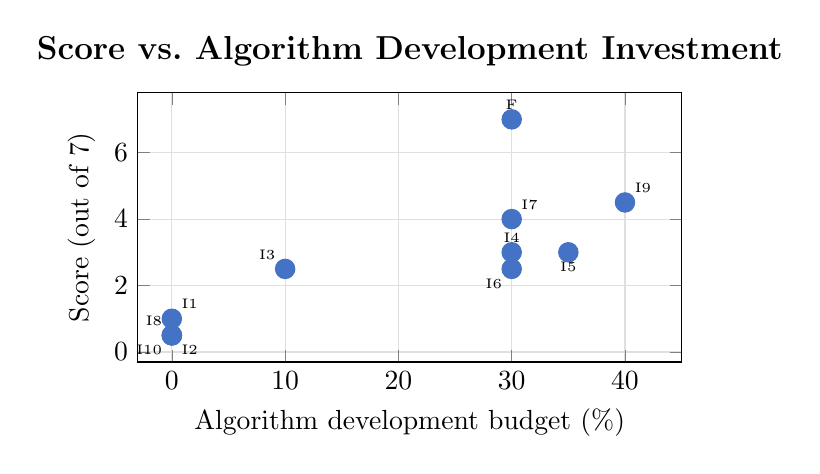
\begin{tikzpicture}
\begin{axis}[
    only marks,
    width=0.70\textwidth,
    height=5cm,
    xlabel={Algorithm development budget (\%)},
    ylabel={Score (out of 7)},
    xmin=-3, xmax=45,
    ymin=-0.3, ymax=7.8,
    ymajorgrids=true,
    xmajorgrids=true,
    grid style={gray!25},
    title={\textbf{Score vs.\ Algorithm Development Investment}},
    title style={font=\large},
    mark size=3pt,
]
\addplot[mark=*, cblue, mark size=3.5pt] coordinates {
    (0,1) (0,0.5) (10,2.5) (30,3) (35,3)
    (30,2.5) (30,4) (0,0.5) (40,4.5) (0,0.5)
    (30,7)
};
% Labels
\node[font=\tiny, above right] at (axis cs:0,1) {I1};
\node[font=\tiny, below right] at (axis cs:0,0.5) {I2};
\node[font=\tiny, above left] at (axis cs:10,2.5) {I3};
\node[font=\tiny, above] at (axis cs:30,3) {I4};
\node[font=\tiny, below] at (axis cs:35,3) {I5};
\node[font=\tiny, below left] at (axis cs:30,2.5) {I6};
\node[font=\tiny, above right] at (axis cs:30,4) {I7};
\node[font=\tiny, above left] at (axis cs:0,0.5) {I8};
\node[font=\tiny, above right] at (axis cs:40,4.5) {I9};
\node[font=\tiny, below left] at (axis cs:0,0.5) {I10};
\node[font=\tiny, above] at (axis cs:30,7) {F};
\end{axis}
\end{tikzpicture}
\caption{Scatter plot of solution quality score against the fraction
  of token budget devoted to algorithm development. Two distinct
  clusters are visible: non-coding attempts at (0\%, 0.5--1) and
  coding attempts at (30--40\%, 2.5--7).}
\label{fig:scatter}
\end{figure}


%% ═══════════════════════════════════════════════════════════════
\section{Aggregate Statistics}\label{sec:stats}

\begin{table}[H]
\centering
\caption{Summary statistics across all 11 attempts.}
\label{tab:aggregate}
\begin{tabular}{@{}lr@{}}
\toprule
\textbf{Metric} & \textbf{Value} \\
\midrule
Total attempts & 11 \\
Total transcript lines (Iter\,1--10) & 26\,128 \\
Mean transcript length & 2\,613 lines \\
Shortest transcript & 1\,909 lines (Iter\,8) \\
Longest transcript & 3\,235 lines \\[3pt]
\midrule
Correct answers & 1 / 11 (9.1\%) \\
Code submissions & 6 / 11 (54.5\%) \\
Heuristic submissions & 3 / 11 (27.3\%) \\
Zero submissions & 2 / 11 (18.2\%) \\[3pt]
\midrule
Mean score (Iter\,1--10) & 2.20 / 7 (31.4\%) \\
Mean score (all 11) & 2.68 / 7 (38.3\%) \\
Median score (Iter\,1--10) & 2.50 / 7 \\
Score std.\ deviation (Iter\,1--10) & 1.42 \\[3pt]
\midrule
Steps with 100\% engagement & 2 (S1, S2) \\
Steps with ${<}20\%$ full discovery & 4 (S3, S4, S5, S7) \\
Hardest step (lowest discovery) & S7 (1/11 full, 1/11 partial) \\
Mean code-submitter score & 3.4 / 7 \\
Mean non-code-submitter score & 0.6 / 7 \\
Closest wrong answer (relative error) & 6.4\% (Iter\,10) \\
\bottomrule
\end{tabular}
\end{table}


%% ═══════════════════════════════════════════════════════════════
\section{Conclusions}\label{sec:conclusions}

\begin{enumerate}
  \item \textbf{Partial coverage is high; full synthesis is rare.}
    Across 11 attempts, the model collectively engaged with all 7
    solution steps. Steps S1--S2 were universally attempted; S3--S6
    were partially discovered by a majority. Yet only 1 attempt
    assembled all pieces correctly, with only 1 of 11 runs
    succeeding.

  \item \textbf{The bottleneck is S7 (global cancellation).}
    This step requires recognising a structural symmetry that
    simplifies the entire computation. It represents a qualitatively
    different type of mathematical insight---a ``cancellation at
    scale'' argument---that the model fails to discover independently.

  \item \textbf{Code submission is a strong positive signal.}
    Code-submitting iterations scored $5.7\times$ higher on average
    than non-code iterations. Writing executable code forces concrete,
    testable reasoning and prevents the drift into unverifiable
    heuristics.

  \item \textbf{Depth beats breadth.}
    Iterations pursuing 2--3 strategies deeply outperformed those
    sampling many strategies superficially. The model's generative
    breadth---its ability to propose diverse approaches---is a
    strength, but without the disciplined depth to follow through,
    it leads to diffuse, low-scoring attempts.

  \item \textbf{Self-calibration is poor.}
    The model expresses uncertainty uniformly, regardless of whether
    its answer is correct. This limits the value of confidence
    signals for downstream evaluation.

  \item \textbf{The last-mile problem is the central challenge.}
    The model can generate the right mathematical framework---the
    right conjectures, the right structural decompositions, the
    right algorithmic skeletons---but cannot reliably close the
    gap between framework and verified computation. Bridging this
    gap likely requires either (a)~integrated verification tools
    (code execution with feedback) or (b)~access to prior
    successful attempts.
\end{enumerate}


\end{document}
